\section{FUNDAMENTAÇÃO TEÓRICA}

De uma maneira simplificada, teoria é aquilo que explica porque algo é como é. Esta seção, deve descrever os conceitos necessários para explicar as decisões a serem tomadas no desenvolver da pesquisa.

Antes de se iniciar as subseções é preciso fazer uma breve apresentação das subseções seguintes, com um bom encadeamento lógico relacionando-as.

Usar diferentes seções para diferentes conceitos-chave do trabalho. Um ponto de partida é considerar três conceitos chave extraídos do título do trabalho.

\subsection{Conceito chave-1}

O que é manga? Fruta, parte da roupa, ou um verbo?

Em cada subseção, é preciso informar ao leitor qual o significado adotado para cada conceito utilizado na pesquisa. Conceitue ou descreva cada um deles. Caso existam diferentes abordagens para um mesmo conceito, deixe claro qual aquela que será adotada.

A fundamentação teórica/revisão bibliográfica não é uma lista de verbetes com explicações. Não basta dizer o que é cada peça usada na montagem do trabalho; tem-se que explicar a função de cada uma e como ela interage com as outras peças. Ao final de cada seção, é preciso informar ao leitor a relação daquele conceito com o trabalho. 

\subsection{Conceito chave-2}

Convém ser caridoso com o leitor: usar uma escrita didática, com boas explicações; o leitor merece reconhecimento por se dispor a conhecer o trabalho, além do fato de que nem sempre entende bem do conteúdo lido.  Revisar, revisar, revisar, pelo menos três vezes, nunca é demais. Evita-se resumir capítulos de livros: uma boa fundamentação apresenta os conceitos relevantes para o trabalho e faz as conexões entre eles. 

O conteúdo de sites como Wikipédia e blogs não são reconhecidos como cientificamente válidos porque seu conteúdo nem sempre é confiável. Usa-se anais de eventos, bons livros, periódicos, bancos de teses e dissertações. Para buscas na internet, sugere-se usar o buscador Google Acadêmico, indexadores como Scielo e BDBComp, o Portal de Periódicos Capes.

Uma forma prática de encontrar os primeiros materiais é procurar nos anais de importantes conferências da sua área de estudo, ou em periódicos relacionados. É comum se precisar de ajuda do orientador para definir quais os principais eventos e periódicos tratam do tema de estudo.

\subsection{Conceito chave-3}

Um texto pode conter diferentes tipos de ilustração, que são: uma "designação genérica de imagem que ilustra ou elucida um texto. São consideradas ilustrações: desenho, esquemas, fluxograma, gráfico, mapa, organograma, planta, quadro, retrato, figura, imagem, entre outros" ~ \cite{ufc_guia}. Todos eles podem ser rotulados pela palavra "Figura", como na Figura 1, ou receber denominações específicas como no Quadro 1. 
Usa-se a denominação Tabelas, que tem formatação específica, apenas em caso de dados numéricos. Quando se tratar de dados textuais, deve-se denominar Quadro.

Usa-se a denominação Tabelas, que tem formatação específica, apenas em caso de dados numéricos. Quando se tratar de dados textuais, deve-se denominar Quadro.

\begin{figure}[H] %use h para forçar que a figura fique abaixo do texto
	\caption{\label{fig:exemplo-1} Exemplo de formatação de figura}
	\begin{center}
	    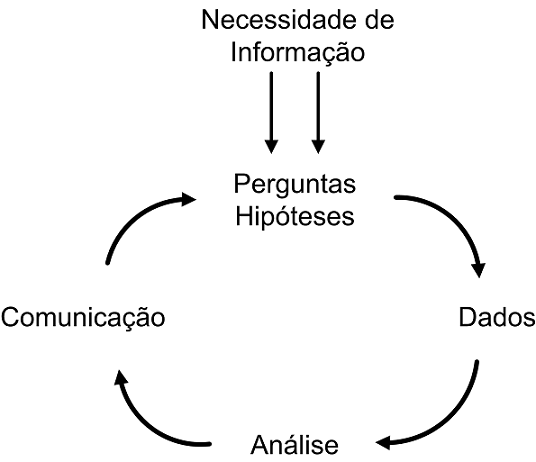
\includegraphics[scale=0.2]{figuras/figura_1} % altere o atributo scale para o tamanho da figura
	\end{center}
	\legend{Fonte: \citeonline{portal_action}}
\end{figure}